\chapter{¿Será estable un gran sistema complejo?}

\section{Sistema de especies en competencia.}

El sistema de Lotka-Volterra de especies en competencia es una de las grandes extensiones del \textit{modelo logístico} aplicado a $N$ especies lo que se traduce en $N$ ecuaciones diferenciales. Es uno de los sistemas más utilizados para poder comprender la naturaleza de la dinámica no lineal; en este sistema se exploran espacios fase más complejos con múltiples puntos fijos y por lo tanto una estabilidad que no es trivial de determinar. Los términos no lineales de estas ecuaciones son cuadráticos y representan la interacción entre la especie $i$ y la especie $j$. El conjunto de ecuaciones diferenciales que representa al sistema es el siguiente:
\begin{equation}\label{eqn:LK}
	\frac{dx_i}{dt}=r_ix_i\left(1-\frac{\sum_{j=1}^N \alpha_{ij}x_j}{K_i}\right)
\end{equation}
Donde $i\in\{1,...,N\}$, las ecuaciones consideran una tasa de crecimiento $r_i$ para la especie $i$, una capacidad de carga $K_i$ que limita hasta cierto punto su crecimiento tal y como se discutió en el capítulo anterior, y se considera su respectiva interacción con la especie $j$ dado por el término $x_ix_j$ cuya ``fuerza'' de interacción esta dada por los coeficientes $\alpha_{ij}$. En un primer acercamiento, cuando nos referimos a ``fuerza'' de interacción nos referimos a la capacidad de la especie $j$ de intervenir sobre la especie $i$, entre más grande sea su coeficiente más afecta a la dinámica de la especie $i$.\\
\\
Como bien sabemos hasta ahora, el sistema llega a ser tan complejo debido a los términos no lineales que ya no es posible poder acceder a una solución analítica general de manera directa o trivial, ya que podrían existir múltiples de ellas tal y como se discutía en el capítulo anterior con base en el teorema de existencia y unicidad\footnote{Referenciar teorema de nuevo.}; para fines de este trabajo únicamente nos concentraremos en las soluciones aproximadas dadas por integración numérica, particularmente con RK4 por su precisión garantizada\footnote{Puedes consultar su implementación en el apéndice, sección (\ref{sec:algoritmos}).}.
\section{Caso particular para $N=2$}

Conviene resolver y analizar el sistema para 2 especies y con base en su experiencia poder extender los aprendizajes al caso generalizado de $N$ especies. Las ecuaciones de (\ref{eqn:LK}) se reducen al siguiente sistema:
$$
\begin{cases}
	\dot{x}_1&=r_1x_1\left (1-\frac{a_{11}x_1}{k_1}-\frac{a_{12}x_1x_2}{k_1}\right )\\
	\dot{x}_2&=r_2x_2\left (1-\frac{a_{21}x_1x_2}{k_2}-\frac{a_{22}x_2}{k_2}\right )
\end{cases}
$$
Para este caso particular y en general, normalmente se tendrá una tasa de crecimiento y una capacidad de carga personalizada para cada especie, lo que es razonable con el hecho de que cada especie crece a un ritmo determinado y también es limitada de manera determinada. Por otro lado, los coeficientes $\alpha_{ij}$ formarán parte de una \textit{matriz de incidencias} entre especies definida de la siguiente manera
\begin{equation}\label{eqn:mIncidencias}
	A=
	\begin{pmatrix}
		1 & \alpha_{12}\\
		\alpha_{21} &1
	\end{pmatrix}
\end{equation}
Es apreciable que los términos de la diagonal se encuentran fijados en $\alpha_{ii} = 1$ respectivamente, más adelante se discutirá sobre esta característica y se dará una explicación detallada del por qué debe ser así, por el momento solo nos enfocaremos en la dinámica que produce el sistema. 

\begin{ejemplo}\label{eg:2x2}
	Para ello definimos el siguiente sistema de especies en competencia
	\begin{equation}\label{eqn:Sist2x2Comp}
		\begin{split}
			\frac{dx}{dt}&=2x\left(1-\frac{x}{2}\right)-xy\\
			\frac{dy}{dt}&=3y\left(1-\frac{y}{3}\right)-2xy
		\end{split}
	\end{equation}
	De este sistema se pueden notar algunas características: se tiene para cada especie una tasa de crecimiento y una capacidad de carga específica o personalizada. Por ejemplo para la ecuación $\dot{x}$ se tiene una tasa de crecimiento y capacidad de carga de 2 para la especie $x$ y para la especie $y$ estos valores son iguales a 1; para la ecuación $\dot{y}$ se tiene una tasa de crecimiento y capacidad de carga de 3 para la especie $x$ y para la especie $y$ se tiene una tasa de crecimiento de 2 y una capacidad de carga de 1. \\
	\\
	Aunque este sistema tal cual no tiene una solución analítica, si es posible explorar acerca de su comportamiento. En principio se pueden hallar sus puntos fijos que nos hablan de la estabilidad del sistema. Para hallar puntos fijos es necesario encontrar las raíces de este sistema. La solución trivial siempre será $(0,0)$, de ahí se tienen que igualar a cero las ecuaciones para hallar los otros puntos críticos.
	\begin{align*}
		2x-x^2-xy &= 0,\qquad\text{suponiendo que $y = 0$}\\
		2x &= x^2\\
		x&=2
	\end{align*}
	y para $\dot{y}$ se tiene
	\begin{align*}
		3y-y^2-2xy&=0,\qquad\text{suponiendo que $x=0$}\\
		3y &= y^2\\
		y &= 3
	\end{align*}
	Por tanto tenemos para $\dot{x}$ el punto fijo $(2,0)$ mientras que para $\dot{y}$ se tiene el punto fijo $(0,3)$. Aún es posible hallar un último punto fijo que es para cuando ambas ecuaciones se hacen cero.
	\begin{align*}
		2x-x^2-xy&=0,\qquad\text{Se despeja $y$ de esta ecuación.}\\
		xy &= x(2-x)\\
		y &= (2-x)\\
		\\
		3(x-2)-(x-2)^2-2x(x-2) &= 0\\
		3x-6-(x^2-4x+4)-2x^2+4x&=0,\qquad\text{Reduciendo términos se tiene.}\\
		x^2-3x+2 &= 0
	\end{align*}
	%%%%%%%%%%%%%%%%%%%%%CHECKPOINT
	Al resolver esta última ecuación y sustityendo en $y$ se encuentra que el último punto fijo que corresponde a $(1,1)$. Como podemos ver ya no solo tenemos 2 puntos fijos (como en el sistema presa-depredador (\ref{eqn:PresaDepredador})) sino hasta 4 puntos fijos y estos irán aumentando de acuerdo al número de especies consideradas. Sus estabilidades pueden ser variadas pero para este caso  veremos que se tendrá un repulsor (el origen), dos atractores (los puntos que se sitúan en los ejes) y un punto silla (el último que determinamos). 
	\\
	\\
	Dependiendo de la elección de condiciones iniciales es la forma en la que va a evolucionar el sistema, en esencia se tienen dos opciones generales, o converge a un atractor de un eje o al otro, donde cada eje corresponde a una especie y por lo tanto la predominancia de una se traduce en la extinción de la otra. Lo dicho hasta este punto lo podremos sustentar a través de un gráfico de espacio fase (Figura (\ref{fig:CompetenciaEspecies})), sin embargo más adelante veremos una técnica para poder conocer la estabilidad de los puntos fijos de forma analítica ya que no siempre podremos contar con la herramienta visual/cualitativa; cuando se tengan más de 3 especies, el espacio fase es $N-$dimensional y por lo tanto imposible de representar.
	\newpage
	
\end{ejemplo}
\begin{wrapfigure}{r}{0.5 \textwidth} \vspace{-30pt} \begin{center}
		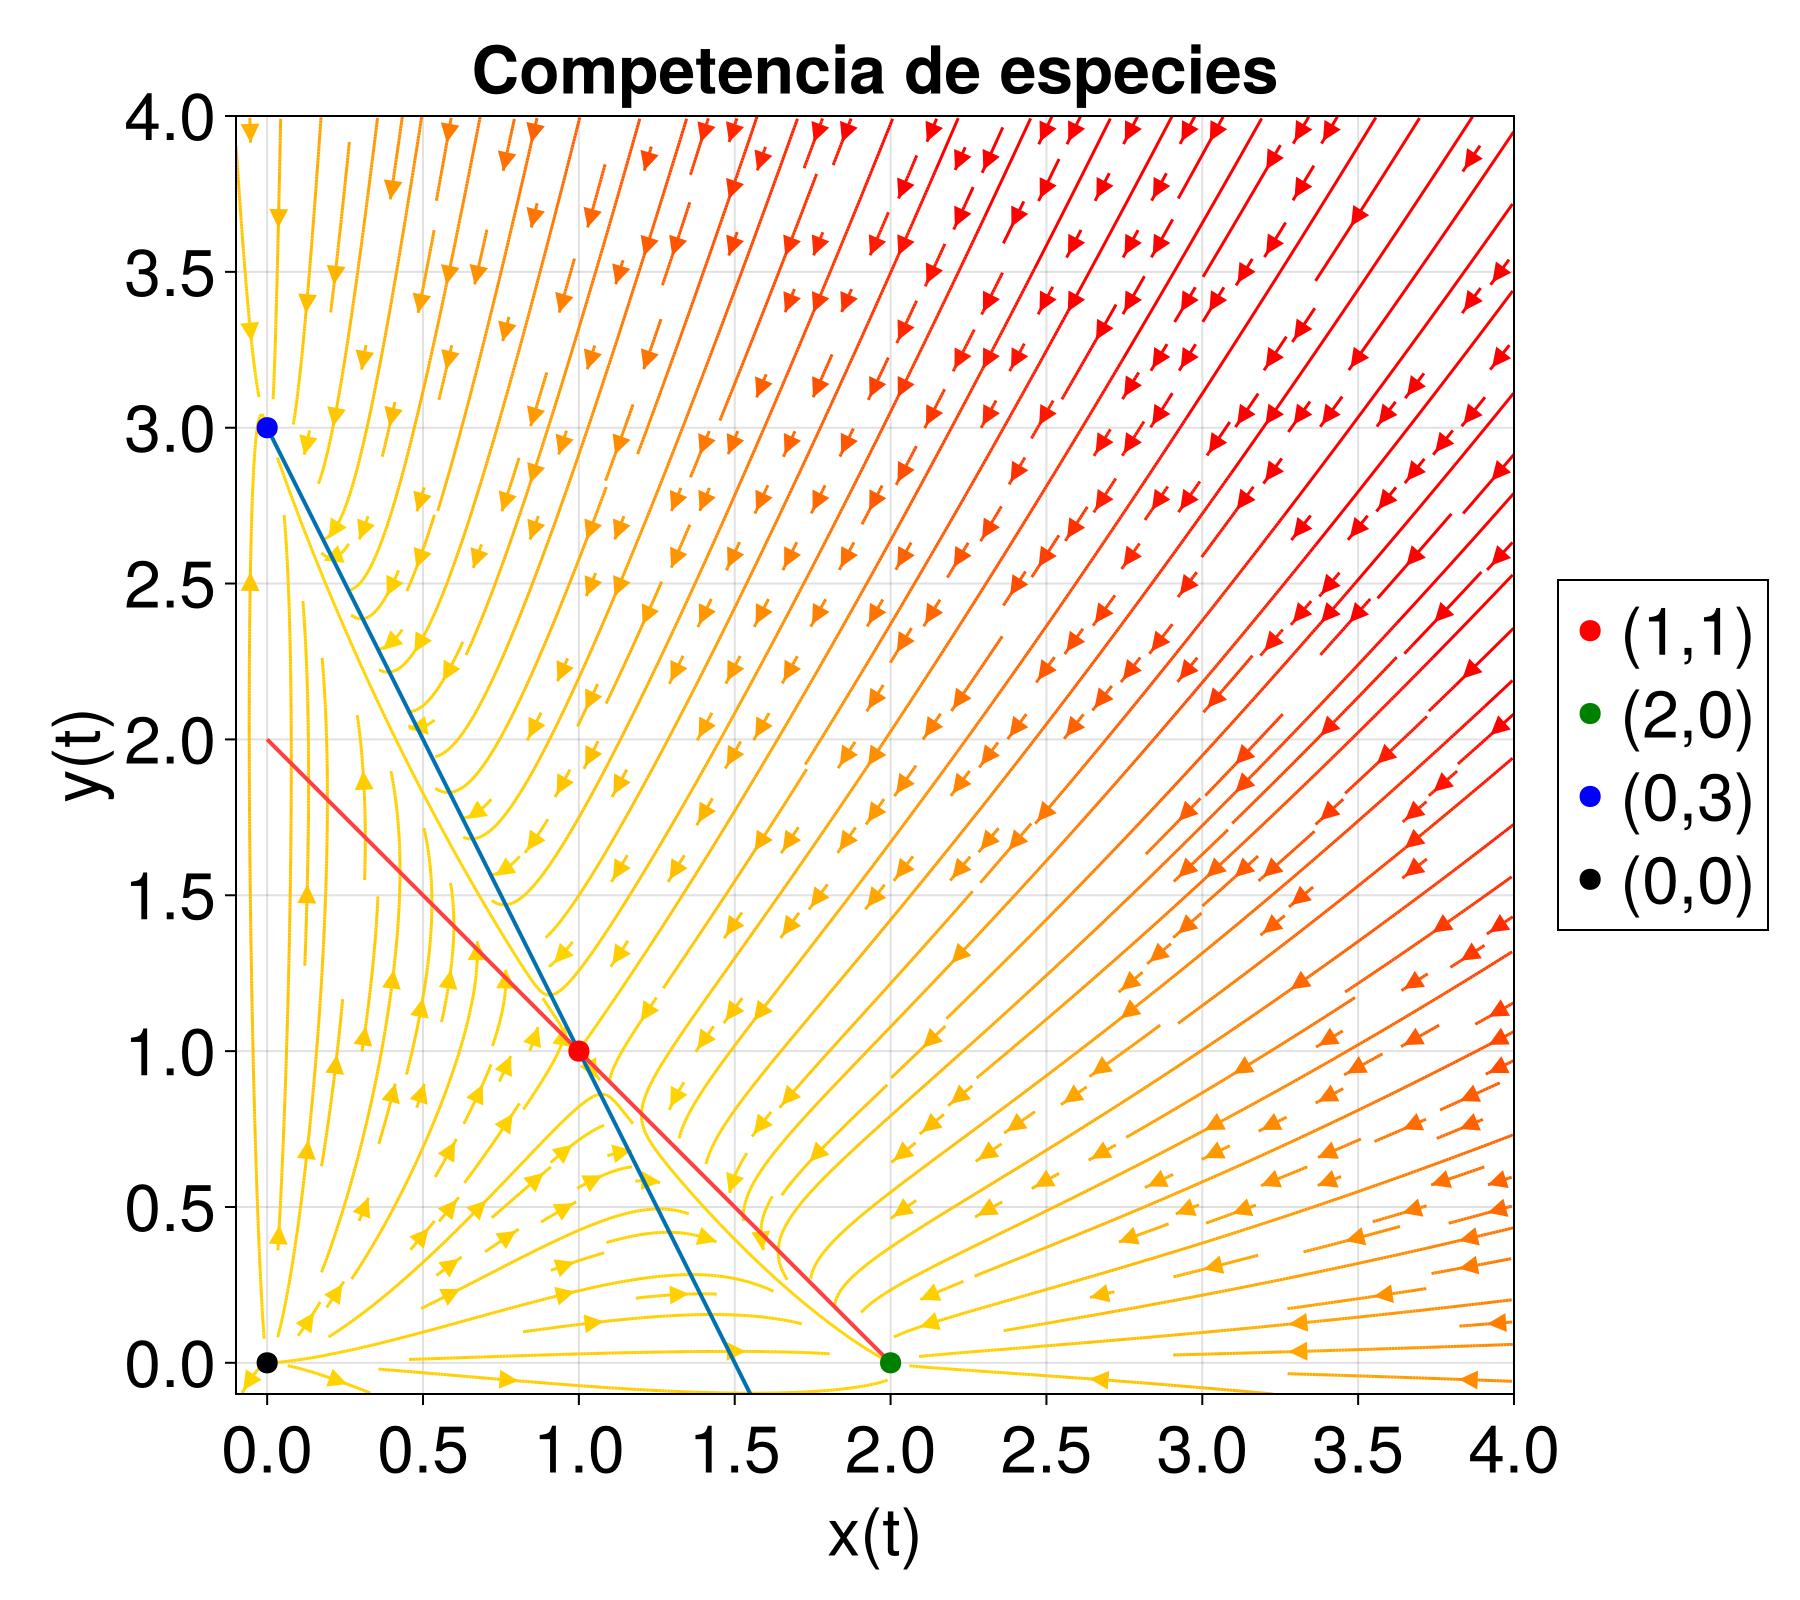
\includegraphics[width=0.5\textwidth]{../Imagenes/Competencia de especies} 
	\end{center} 
	\vspace{-20pt} 
	\caption{Campo vectorial de las soluciones del sistema propuesto de dos especies.} 
	\vspace{-10pt}
	\label{fig:CompetenciaEspecies}
\end{wrapfigure} 
\setlength{\parindent}{0cm}Una vez determinando el espacio fase del sistema, podemos comprobar la estabilidad de los puntos fijos antes encontrados, de tal modo que todas las posibles soluciones terminan convergiendo a uno de los dos atractores posibles. Además de ello podemos observar las dos isoclinas del sistema que no son más que el conjunto de puntos donde se satisface:
\begin{equation*}
	\dot{x}=f(x,y)=0,\qquad\dot{y}=g(x,y)=0
\end{equation*}
a lo largo de la isoclina de $x$ la componente en $x$ es cero y sus soluciones únicamente apuntarán hacia arriba o hacia abajo, dependiendo de la zona. De modo similar ocurre para la isoclina de $y$, en donde la componente $y$ es cero y sus sus soluciones a lo largo de la recta solo pueden ir hacia la derecha o izquierda de forma horizontal. Nuevamente podemos apreciar al punto silla como inestable ya que posicionados ahí y ante una mínima perturbación, el sistema se alejará de este punto e irá convergiendo a cualquiera de los dos atractores (dependiendo de la perturbación). Por último es bien sabido que del origen todas las soluciones divergen debido a la tasa de crecimiento que genera un aumento natural en las poblaciones.\\
\\
%%%%%%%%%%%%%%%%%%%%%CHECKPOINT
%% Nada más checar la aseveración de las isoclinas para ver si se queda o se retira del párrafo
Al tratarse de un sistema simple de dos ecuaciones, se tiene la fortuna poder contar con el espacio fase que nos brinda información crucial sobre su estabilidad, pero ¿Qué ocurre cuando tenemos un sistema de más de 3 especies? como se ha mencionado, la representación visual ya no esta disponible porque cada eje del espacio fase representa a una de las especies que intervienen. A lo mucho podemos acceder a sub-espacios del hiper-espacio fase pero además de que sería engorrosa la generación de cada gráfica, al final solo obtendríamos información a nivel local. 
\\
\\
Si el número de ecuaciones del sistema (\ref{eqn:LK}) llega a ser considerablemente alto, conviene mejor ejecutar una técnica analítica para poder conocer la estabilidad de cada uno de los puntos fijos del sistema, a dicha técnica se le conoce como \textit{linealización}\footnote{agregar referencia}. Particularmente para nuestro sistema, el proceso consiste en bajar el grado de las ecuaciones no lineales para convertirlo a un sistema lineal, y poder operar como se hizo en el capítulo anterior. Los términos no lineales de nuestro sistema (\ref{eqn:LK}) son cuadráticos y basta con bajarles su grado por medio de derivadas parciales. Por lo tanto el proceso de linealización consiste en convertir el sistema (\ref{eqn:LK}) en un sistema lineal aplicándole el \textit{jacobiano}.
\newpage
\begin{definición}\label{def:LKVectorial}
	Sea la función vectorial $\mathbf{F}:\mathbb{R}^n\to\mathbb{R}^n$, entonces el sistema de Lotka-Volterra de especies en competencia se define en su forma vectorial del la siguiente manera
	\begin{equation}\label{eqn:Fmatricial}
		\mathbf{F}(\vec{x})=\begin{pmatrix}
			f_1(\vec{x})\\
			\vdots\\
			f_n(\vec{x}))
		\end{pmatrix},\qquad\text{donde $\vec{x}(t)=\left(x_1(t),...,x_n(t))\right)\in\mathbb{R}^n$.}
	\end{equation}
	donde cada una de las componentes de $\mathbf{F}(\vec{x})$ corresponde con las funciones del sistema (\ref{eqn:LK}), mientras que las componentes del vector $\vec{x}$ corresponden con las especies involucradas. Por lo tanto el sistema (\ref{eqn:LK}) puede ser re-escrito de la siguiente forma
	\begin{equation}\label{eqn:LKmatricial}
		\dot{X}(t) = \mathbf{F}(X(t)),\qquad\text{considerando $\dot{X}(t)=\frac{d\vec{x}(t)}{dt}$}
	\end{equation}
	Nos conviene definir al sistema de esta manera para que podamos ver directamente como se aplica el Jacobiano 
	\begin{equation}\label{eqn:Jacobiano}
		\mathbb{J}_\mathbf{F}(\vec{x}) = \begin{pmatrix}
			\frac{\partial f_1(\vec{x})}{\partial x_1} & \cdots &\frac{\partial f_1(\vec{x})}{\partial x_n}\\
			\vdots & \ddots & \vdots\\
			\frac{\partial f_n(\vec{x})}{\partial x_1} & \cdots &\frac{\partial f_n(\vec{x})}{\partial x_n}
		\end{pmatrix}
	\end{equation}
	El jacobiano resultante al ser evaluado en los puntos fijos del sistema es ahora un sistema lineal al que le podemos extraer sus eigenvalores para poder conocer su estabilidad. Esta matriz es conocida como \textit{matriz de interacciones} ya que guarda en ella la información necesaria para determinar la estabilidad de los puntos fijos del sistema. Sin embargo esta información también se esta limitada a nivel local, pues no será posible que nos brinde información de algún  otro punto fijo.
\end{definición}

\setlength{\parindent}{0cm}Para validar esta aseveración continuaremos con nuestro ejemplo y determinaremos la estabilidad de cada uno de los puntos fijos relacionándolos con lo mostrado en el espacio fase. Para ello aplicamos el jacobiano al sistema de ecuaciones quedándonos con:
\begin{equation}\label{eqn:Jacobiano2}
	\mathbb{J}_\mathbf{F}(\vec{x})=\begin{pmatrix}
		r_1-\frac{2r_1x_1+r_1a_{12}x_2}{K_1} & -\frac{r_1a_{12}x_1}{K_1}\\
		-\frac{r_2a_{21}x_2}{K_2} & r_2-\frac{2r_2x_2+r_2a_{21}x_1}{K_2}
	\end{pmatrix}
\end{equation}
debido a la matriz de incidencias (\ref{eqn:mIncidencias}), se tiene que los valores de la diagonal son $a_{ii}=1$ y corresponden con las auto-interacciones del sistema. Sustituyendo y operando sobre nuestro sistema, al evaluar los puntos fijos antes encontrados se tienen las siguientes matrices de interacciones:
$$
\mathbb{J}_{(2,0)} = \begin{pmatrix}
	-2 & -2\\
	0 & -1
\end{pmatrix},\qquad \mathbb{J}_{(0,3)}=\begin{pmatrix}
	-1 & 0\\
	-6 & -3
\end{pmatrix},\qquad \mathbb{J}_{(1,1)}=\begin{pmatrix}
	-1 & -1\\
	-2 & -1
\end{pmatrix},\qquad \mathbb{J}_{(0,0)}=\begin{pmatrix}
	2 & 0 \\
	0 & 3
\end{pmatrix}
$$
%%%%%%%%Checkpoint
Como previamente se ha revisado, los eigenvalores determinan la estabilidad de un sistema lineal. Se establece que mientras ellos tengan parte real negativa se asegurará que el punto fijo será estable y que en otro caso será inestable. Por lo tanto los eigenvalores de las primeras dos matrices de interacciones deben ser negativos para que sustenten los atractores de la figura (\ref{fig:CompetenciaEspecies}). Mientras que los eigenvalores de $\mathbb{J}_{(1,1)}$ deben ser uno negativo y otro positivo para sustentar al punto silla. Para el caso de la matriz $\mathbb{J}_{(0,0)}$ sus eigenvalores deben tener parte real positiva para que sustenten el repulsor. Realizando el álgebra correspondiente se encuentra lo siguiente
\begin{align*}
	\mathbb{J}_{(2,0)}&\Longrightarrow\ \lambda_1 = -2,\quad\lambda_2 = -1\\
	\mathbb{J}_{(0,3)}&\Longrightarrow\ \lambda_1 = -3,\quad\lambda_2 = -1\\
	\mathbb{J}_{(1,1)}&\Longrightarrow\ \lambda_1 = -1+\sqrt{2},\quad\lambda_2 = -1-\sqrt{2}\\
	\mathbb{J}_{(0,0)}&\Longrightarrow\ \lambda_1 = 2,\quad\lambda_2 = 3\\
\end{align*}
Por tanto se termina de validar la consistencia del método de la linealización al menos para este caso particular. Esta técnica resulta muy útil para obtener la estabilidad de los puntos fijos de forma analítica sin tener que recurrir a una representación visual y como bien se ha mencionado, sobre todo para cuando tengamos sistemas $N$ ecuaciones diferenciales en donde los espacios fase ya son $N$-dimensionales. En la siguiente sección se estará generalizando todo lo mencionado hasta ahora para cuando se tenga dicho escenario.

%%%%%%%%% Checkpoint
\section{Generalizando a N especies}

En la sección anterior se ha introducido el sistema de especies en competencia (\ref{eqn:LK}) y se ha definido su forma vectorial (\ref{eqn:LKmatricial}) generalizada; se mostró un ejemplo particular con $n=2$ para observar su dinámica a través de su espacio fase (figura (\ref{fig:CompetenciaEspecies})) en donde se contempla la naturaleza de sus puntos fijos si se trata de atractores, repulsores o puntos silla. Se propone el método de la linealización para conseguir matrices de interacción que determinen de forma analítica la estabilidad de cada uno de los puntos fijos del sistema. En esta sección se profundizará más acerca de lo mencionado comenzando con la construcción matriz de incidencias que será eje fundamental de las interacciones del sistema de $N$ especies. \\
\\
Hasta ahora se ha estado discutiendo puramente sobre dinámica y ecuaciones diferenciales, sin embargo, el lector recordará al principio del primer capítulo que se ha mencionado sobre el uso estratégico de redes para poder modelar cierto sistema dinámico no lineal, en este caso para representar las interacciones de (\ref{eqn:LK}): por lo tanto, ahora toca hablar un poco sobre redes. Una red es considerada una colección de \textit{nodos} que se encuentran unidos por \textit{enlaces}\footnote{definir más adelante el tipo de interacciones con base en el signo y si son dirigidas o no dirigidas. Además de agregar cita del Newman para esta definición.}. Para definir redes siempre es necesario establecer que es lo que representan los nodos y que representan los enlaces, en nuestro caso los nodos representan directamente las especies que participan en el sistema mientras que los enlaces serían sus interacciones, más adelante veremos su naturaleza.\\
\\
Si definimos un conjunto de especies $x_i$ y sabemos que se relacionan por medio de los coeficientes $\alpha_{ij}$ de 
\begin{wrapfigure}{l}{0.45 \textwidth} \vspace{-30pt} \begin{center}
		\includesvg[width=.5\textwidth]{../Imagenes/karateLu} 
	\end{center} 
	\vspace{-20pt} 
	\caption{Red de Karate de Zachary} 
	\vspace{-20pt}
	\label{fig:RedKarate}
\end{wrapfigure} 
(\ref{eqn:LK}), entonces decimos que una interacción entre las especies $x_i$ y $x_j$ (nodos de la red) es para cuando $\alpha_{ij}\neq 0$ y esto representaría un enlace en la red. En el mundo es posible encontrar diferentes tipos de redes con cierto significado, tales como la red de energética de un país, redes de amistades en una universidad o redes de acciones que cotizan en la bolsa de valores; en el caso de la Figura (\ref{fig:RedKarate}) es una red conocida por quienes se dedican a ello y es la representación de una red social llamada \href{https://en.wikipedia.org/wiki/Zachary%27s_karate_club}{Red del club Karate de Zachary}. Para poder representar estas redes y cualquier otro tipo de red conviene introducir el concepto de \textit{matriz de adyacencia.}
\begin{definición}\label{def:matrizdeadyacencia}
	Sea $A\in\mathcal{M}_n(\mathbb{R}) $. Se define la matriz de adyacencia tal que sus entradas son de la siguiente forma
	$$a_{ij}= 
	\begin{cases}
		1, \ \text{si $\exists$ un enlace entre el nodo $i$ y el nodo $j$.}\\
		0, \ \text{en otro caso}.
	\end{cases}$$
	La matriz de adyacencia será la herramienta para determinar la relación de interacción entre especies, pero solo hablará de su existencia y se tendrán que agregar algunas características para darle los pesos de interacción, mismos que están representados por los coeficientes $\alpha_{ij}$ del sistema (\ref{eqn:LK}) 
\end{definición}
%%%%%%% Checkpoint
\begin{ejemplo}
	Para poder apreciar la matriz de adyacencia definamos una red de 10 nodos y veamos la matriz de adyacencia que le corresponde. Cada nodo ha sido marcado para poderlo identificar y relacionar con la matriz de adyacencia. Los renglones y columnas de la matriz representan los nodos, siendo el primer renglón el primer nodo (número 1), el quinto renglón será el quinto nodo (número 5); esto pasa de manera equivalente con las columnas, la cuarta columna corresponde con el cuarto nodo (número 4), la octava columna corresponde con el octavo nodo (número 8). Por tanto, mediante la matriz de adyacencia sabemos que el primer nodo (renglón 1) esta enlazado con el noveno nodo (columna 9) ya que existe un uno, mientras que el primer renglón y la quinta columna hay un cero lo que indica que no existe un enlace entre estos nodos. 
\end{ejemplo}
\begin{wrapfigure}{r}{0.5 \textwidth} \vspace{-30pt} \begin{center}
		\includesvg[width=0.5\textwidth]{../Imagenes/red10Lu} 
	\end{center} 
	\vspace{-20pt} 
	\caption{Red no dirigida de 10 nodos.} 
	\vspace{-150pt}
	\label{fig:Red10}
\end{wrapfigure} 

$$
A=\begin{pmatrix}
	0 & 1 & 0 & 1 & 0 & 0 & 0 & 0 & 1 & 0 \\
	1 & 0 & 1 & 0 & 0 & 1 & 0 & 0 & 0 & 0 \\
	0 & 1 & 0 & 0 & 0 & 0 & 1 & 1 & 0 & 0 \\
	1 & 0 & 0 & 0 & 1 & 1 & 1 & 0 & 0 & 1 \\
	0 & 0 & 0 & 1 & 0 & 0 & 0 & 0 & 1 & 1 \\
	0 & 1 & 0 & 1 & 0 & 0 & 1 & 1 & 0 & 1 \\
	0 & 0 & 1 & 1 & 0 & 1 & 0 & 0 & 1 & 0 \\
	0 & 0 & 1 & 0 & 0 & 1 & 0 & 0 & 1 & 0 \\
	1 & 0 & 0 & 0 & 1 & 0 & 1 & 1 & 0 & 1 \\
	0 & 0 & 0 & 1 & 1 & 1 & 0 & 0 & 1 & 0 \\
\end{pmatrix}
$$
También hay que destacar qué la matriz es simétrica y que la diagonal es igual a cero: para el primer punto se debe notar que la relación de los enlaces entre nodos no tiene dirección, es decir, que exista un enlace entre nodos significa que el nodo $i$ se conecta con $j$ y viceversa, que el nodo $j$ se conecta con el nodo $i$. Por tanto decimos que la red de la figura (\ref{fig:Red10}) es \textit{no dirigida} puesto que no hay una dirección preferencial en el enlace. Para el segundo punto se puede deducir que los nodos podrían relacionarse consigo mismo, en este caso caso particular no lo hacen pero si es posible la existencia de \textit{autoenlaces}. Para el sistema (\ref{eqn:LK}) los autoenlaces representan las autointeracciones que dan el caracter logístico de las ecuaciones. En cuanto se defina la matriz de interacciones se verá el papel que toman los elementos de la diagonal y de porque deben de existir autoenlaces en cada una de las ecuaciones del sistema.	
\\
\\
Cuando se tiene el caso en que los enlaces tienen una dirección preferencial de nodo a nodo, decimos que corresponde a una \textit{red dirigida}. En este caso el enlace podrá ir del nodo $i$ al nodo $j$ pero no necesariamente lo hará en sentido contrario, deberá definirse explícitamente. En el mundo también existe un gran conjunto de redes dirigidas como lo son las citaciones académicas, la propia WWW (World Wide Web), incluso redes tróficas de depredador-presa. Y para este caso también se tiene asociada una matriz de adyacencia con una ligera diferencia con respecto de la definición \ref{def:matrizdeadyacencia}.
\begin{definición}
	Sea $D\in\mathcal{M}_n(\mathbb{R})$, matriz de adyacencia de una red no dirigida. Se definen sus elementos de la siguiente manera:
	$$
	\alpha_{ij}=\begin{cases}
		1,\qquad\text{Si existe un enlace del nodo $i$ al nodo $j$}\\
		0,\qquad\text{otro caso.}
	\end{cases}
	$$
	Los enlaces de las redes dirigidas van a estar representados por flechas para que puedan mostrar adecuadamente las direcciones correspondientes entre los nodos. 
\end{definición}

\begin{ejemplo}
	Se tiene la siguiente red dirigida de 10 nodos con exactamente 14 enlaces. La matriz de adyacencia asociada es la siguiente
\end{ejemplo}

\begin{wrapfigure}{l}{0.5 \textwidth} \vspace{-30pt} \begin{center}
		\includesvg[width=0.52\textwidth]{../Imagenes/Red10DirLu} 
	\end{center} 
	\vspace{-20pt} 
	\caption{Red no dirigida de 10 nodos.} 
	\vspace{-150pt}
	\label{fig:Red10Dir}
\end{wrapfigure} 
$$
D = \begin{pmatrix}
	0 & 0 & 0 & 0 & 0 & 0 & 0 & 0 & 0 & 1 \\
	1 & 0 & 1 & 0 & 0 & 0 & 0 & 1 & 0 & 0 \\
	0 & 0 & 0 & 1 & 1 & 0 & 0 & 0 & 0 & 1 \\
	1 & 0 & 0 & 0 & 0 & 0 & 0 & 0 & 0 & 0 \\
	0 & 0 & 1 & 0 & 0 & 0 & 0 & 1 & 0 & 0 \\
	0 & 1 & 0 & 0 & 0 & 0 & 0 & 0 & 0 & 0 \\
	0 & 0 & 1 & 0 & 0 & 0 & 0 & 0 & 0 & 0 \\
	0 & 0 & 0 & 0 & 0 & 0 & 0 & 0 & 0 & 0 \\
	0 & 1 & 0 & 0 & 0 & 0 & 0 & 0 & 0 & 0 \\
	0 & 0 & 0 & 0 & 0 & 0 & 1 & 0 & 0 & 0 \\
\end{pmatrix}
$$

Ahora se puede notar que la matriz de adyacencia no es simétrica y que por lo tanto los enlaces presentan una dirección preferencial. Ambas visiones se van a tomar en cuenta para modelar al sistema de especies en competencia, sin embargo, preferentemente tendrá mayor protagonismo la \textit{red no dirigida} que la otra ya que como se verá más adelante, producen los mismos resultados y la diferencia recae en el tiempo de obtención de los datos en donde las redes dirigidas requieren mayor tiempo de compilación para generar escenarios estables.\\
\\
En este punto el lector ya debe suponer la razón de la presentación de estas dos formas de redes; el sistema dinámico de especies en competencia considera las interacciones dadas por los coeficientes $\alpha_{ij}$, sin embargo puede que exista el coeficiente $\alpha_{ij}$ que relaciona a la especie $x_i$ con la $x_j$ pero bien podría suceder que $\alpha_{ji}=0$ y en consecuencia no exista interacción de la especie $x_j$ con la especie $x_i$. Por lo tanto la matriz de incidencias, esta construida con base en alguna de estas dos formas de red. 

\subsection{Red de incidencias}

La \textit{red de incidencias} es el artilugio principal que se va a ocupar para poder modelar las interacciones del sistema de especies en competencia, tiene asociada una matriz de adyacencia que llamaremos \textit{matriz de incidencias} y se va a componer de tres factores: puede ser de una red dirigida o no dirigida, las interacciones son importantes y definir la dirección de las mismas hace más completo al sistema, sin embargo usaremos mayormente redes no dirigidas. La topología de la red que se va a utilizar es la conocida \textit{red aleatoria} de Erdös–Rényi [Cita\footnote{poner cita de esto}] que nos van a modelar interacciones entre las especies de forma aleatoria con base en cierto parámetro. Y aunado a todo ello tendremos una matriz de pesos en donde sus entradas se encuentran en una distribución normal centrada en el cero. La conjunción de estos tres elementos da lugar a la matriz de incidencias y por lo tanto a su red asociada.\\
\\
La red de Erdös–Rényi es ampliamente utilizada para aprender sobre la estructura y propiedades de la redes y con ello poder extender ese aprendizaje al estudio de las llamadas \textit{redes libres de escala}. La diferencia sustancial entre la red aleatoria y la red libre de escala es que la primera tiene muy pocas (o ninguna) aplicaciones en escenarios de la naturaleza, se ha encontrado que las estructuras de las redes en la naturaleza siguen cierto patrón y distribución que se han englobado en las redes libres de escala. Sin embargo este trabajo únicamente se centrará en el uso del modelo de Erdös–Rényi aplicado al sistema (\ref{eqn:LK}) para poder entender la dinámica que produce y con las intenciones de extender el análisis al caso de las redes libres de escala\footnote{Un modelo teórico que rescata todas las propiedades de las redes libres de escala es el de Albert-Barabasi [Cita].}. 
\begin{definición}\label{def:redAleatoria}
	Sea un conjunto de $N$ nodos sin enlaces asociados. Para cada par de nodos $i$ y $j$ de las $\binom{N}{2}$ posibles combinaciones, se definen sus enlaces aleatorios dada una probabilidad $p$ y un número aleatorio $r$ en el intervalo $[0,1]$ de la siguiente forma
	$$
	L_{ij}=\begin{cases}
		\exists,\qquad\text{Si }r<p\\
		\nexists,\qquad\text{Si }r\geq p
	\end{cases}
	$$
	desde luego que entre mayor sea la $p$ se tendrá mayor cantidad de enlaces. El conjunto de los $N$ nodos con sus posibles $L_{ij}$ enlaces forman la red aleatoria de Erdös–Rényi. En esta referencia [cita\footnote{referencia a barabasi}] el lector podrá conocer más sobre sus propiedades, nosotros por ahora solamente haremos uso de ella. La matriz de adyacencia de esta red aleatoria es simétrica lo que nos da entender que la red es no dirigida en esencia. Podemos extender esta definición a redes aleatorias dirigidas suponiendo que la conexión va en dirección del nodo $i$ al nodo $j$ y considerar también conexiones del nodo $j$ al nodo $i$, por lo tanto ahora tendremos $N(N-1)$ posibles combinaciones de nodos. \\
	\\
	Si solo se considerara uno de los dos casos, es decir, para $\binom{N}{2}$ combinaciones de nodos entonces tendríamos la mitad de posibles conexiones, la matriz de adyacencia sería triangular superior por haber considerado únicamente la dirección de $i$ a $j$. Para llenar la parte triangular inferior de esta matriz debemos considerar las conexiones de $j$ a $i$ y haciéndolo de esa forma habremos obtenido nuestra red aleatoria dirigida cuya matriz de adyacencia es no simétrica, es decir, que en general se cumple $A_{ij}\neq A_{ji}$. En la sección (\ref{sec:RedesAleatorias}) se encuentra la implementación computacional de ambas visiones de la red aleatoria.
\end{definición}
\newpage
\setlength{\parindent}{0cm}En este punto estamos a un solo paso de construir finalmente a la matriz de incidencias, únicamente nos falta de considerar la magnitud de las interacciones entre especies y para ello se va a emplear una matriz de $N\times N$ donde $N$ es el número de nodos de la red que vayamos a modelar; esta matriz se va a mapear con una función de densidad de probabilidad (FDP) asociada a una distribución normal en cada entrada
$$f(x)=\frac{1}{\sigma\sqrt{2\pi}}e^{-\frac{(x-\mu)^2}{2\sigma^2}}$$
en esencia será una matriz con entradas aleatorias bajo una FDP centrada en $\mu = 0$ y variando a sigma en $[0,1]$ con un paso de $0.1$ (esto se irá detallando más adelante). 
\begin{definición}
	Sea una red aleatoria de $N$ nodos dirigida o no dirigida y $A$ su matriz de adayacencia asociada, definimos así mismo una matriz de entradas aleatorias $M$ mapeada bajo una FDP centrada en $\mu=0$ y con $\sigma\in[0,1]$. Definimos a $\Lambda$ la \textit{matriz de incidencias} como el producto de Hadamard (entrada a entrada) de la matriz de adyacencia con la matriz aleatoria sumada con la matriz identidad:
	\begin{equation}\label{eqn:MatrizIncidencias}
		\Lambda=(A\odot M) + I
	\end{equation}
	El producto $A\odot M$ simplemente agrega pesos a cada posible enlace de a la matriz de adyacencia asociada a la red aleatoria de nuestra elección, y seguida la suma con la identidad es para poder agregar autoenlaces a cada nodo de la red aleatoria.
\end{definición}
\setlength{\parindent}{0cm}La matriz de incidencias $\Lambda$ puede ser \textit{estructuralmente simétrica}\footnote{Es una matriz cuyas entradas cumplen $B_{ij}\neq B_{ji}\neq 0$ para toda $B_{ij}\in B$, quiere decir que aunque $B$ no sea simétrica, relativo a las posiciones de sus entradas si lo es.} si se escoge una red aleatoria no dirigida, o su contraparte si se escoge una red aleatoria dirigida, además para todo $\alpha_{ii}\in\Lambda$, se tiene que 
\begin{wrapfigure}{r}{0.5 \textwidth} \vspace{-30pt} \begin{center}
		\includesvg[width=0.52\textwidth]{../Imagenes/RedIncidencias} 
	\end{center} 
	\vspace{-52pt} 
	\caption{Red de incidencias de 8 nodos bajo la topología de una red aleatoria dirigida con $p=0.15$ y una matriz aleatoria con $\mu=0$ y $\sigma=0.2$.} 
	\vspace{-10pt}
	\label{fig:RedIncidencias}
\end{wrapfigure} 
$\alpha_{ii}=1.0$. Esto nos lleva a asociar esta matriz con una red con pesos y autoenlaces a la que llamaremos \textit{red de incidencias}. Por la forma en como consideramos $M$ para la red de incidencias resultante, decimos que es forzosamente dirigida independientemente de la elección de red aleatoria. Hablando específicamente para el caso en donde se considera $A$ simétrica de la red no dirigida, al momento de realizar el producto punto con $M$, las entradas $\alpha_{ij}$ no necesariamente son iguales a su contraparte simétrica, por lo que se tendrá un peso para el enlace $i\to j$ y otro peso diferente para el enlace $j\to i$; en este caso la matriz podrá ser únicamente estructuralmente simétrica. Para que $\Lambda$ fuera enteramente simétrica necesitaríamos considerar que $M$ estuviera mapeada en la parte triangular superior sus entradas aleatorias y la simetrizáramos hacia su correspondiente triangular inferior, solo así así podríamos conseguir una red de incidencias puramente no dirigida con $\Lambda$ simétrica. La figura (\ref{fig:RedIncidencias}) es una representación visual de los sistemas con los que iremos a trabajar bajo las ecuaciones de (\ref{eqn:LK}). En la sección (\ref{sec:redIncidencias}) se muestra la implementación computacional de la red de incidencias.

\subsection{Tipos de interacciones}

La red de incidencias es de tipo dirigida independientemente de la red aleatoria que se decida elegir para su construcción, a lo mucho podrá ser estructuralmente simétrica pero los pesos de los enlaces $i\to j$ y $j\to i$ son diferentes lo que implica que los coeficientes cumplen $\alpha_{ij}\neq\alpha_{ji}$ para toda $\alpha_{ij}\in\Lambda$. Esto genera repercusiones interesantes para el sistema (\ref{eqn:LK}) por lo que conviene conocer que tipos de interacciones pueden darse en $\Lambda$ y como impactan en la dinámica del sistema.\\
\\
Hasta ahora sabemos que los $\alpha_{ij}\in\Lambda$ forman parte de una FDP centrada en $\mu=0$ y con $\sigma\in[0,1]$, cabe preguntarse si para todo valor posible de $\alpha_{ij}$ tendremos una dinámica homogénea o si se tendrán escenarios particulares. May nos brinda la respuesta [cita\footnote{poner cita  del libro de ecología.}] con un abanico de 5 posibles escenarios. Antes de presentar los escenarios hay que resaltar el hecho de que el signo de $\alpha_{ij}$ importa mucho más que el propio peso que se le asigne, ya que tiene repercusiones en la ecuación (\ref{eqn:LK}) más que nada con el signo negativo de la suma dentro del paréntesis; particularmente si tenemos $\alpha_{ij}<0$ el producto de la especie $x_i$ con la $x_j$ ya no se resta sino lo contrario, de forma que fomenta el propio crecimiento de la especie $x_i$ (suponiendo que nos situamos en la ecuación $\dot{x}_i=f_i(\vec{x})$).\\
\\
El tipo de interacciones a las que May se refiere, aplican a la \textit{community matrix} que es para nosotros la martiz de interacciones, es decir, el Jacobiano del sistema (\ref{eqn:Jacobiano}) evaluado en algún punto fijo estable. Estas interacciones no necesariamente aplican a nuestra matriz de incidencias, de hecho más adelante se discutirá que las interacciones de May aplicarán a la red de incidencias si y solo si las volteamos al signo contrario; y en su momento se verá que al aplicar el Jacobiano a las ecuaciones (\ref{eqn:LK}), las interacciones de las especies cerca del equilibrio se ajustan con lo que May estipula.\\
\\
Las 5 posibles interacciones se reparten de la siguiente forma: para la red de interacciones\footnote{Refiriéndonos a la \textit{community matriz de May}} no dirigida cuya matriz de adyacencia $A$ es estructuralmente simétrica, únicamente puede acceder a dos tipos de interacciones las de competencia $(--)$ y las de mutualismo o simbiosis\footnote{A mi me gusta llamarles de cooperación, así que de ahora en adelante de esa forma me estaré refiriendo a ellas.} $(++)$. Al ser estructuralmente simétrica sus coeficientes cumplen una de las dos situaciones: $A_{ij}\neq A_{ji}\neq 0$ ó $A_{ij}=A_{ji}=0$ para toda $A_{ij}\in A$, lo que significa que si son diferentes de cero tendrán mismo signo y diferentes pesos. Cuando sus signos son positivos implica que la especie $x_i$ y la(s) especie(s) $x_j$ cooperan y fomentan sus crecimientos aunque la medida de ello dependerá de la magnitud de sus pesos asignados. En el caso en donde los signos de las entradas cuasi simétricas sean negativos entonces existe una relación de competencia y la especie $x_i$ compite con la(s) especie(s) $x_j$ de tal forma que una de las especies intentará sobreponerse en las otras. 
\\
\\
Para el caso de la red de interacciones dirigida, pueden acceder a los 5 tipos de interacción ya que en su matriz de adyacencia bien pueden existir entradas cuasi simétricas aunque la matriz en general no lo sea, las que nos faltan son: el comensalismo $(+0)$, amensalismo $(-0)$ y presa-depredador $(+-)$. Para el caso del comensalismo se da para cuando tenemos una interacción de $i\to j$ y la especie $x_i$ obtiene un beneficio mientras que no existe algún impacto para la especie $x_j$. En contraparte el amensalismo es cuando se tiene la interacción $i\to j$ y la especie $x_i$ se ve perjudicada mientras que tampoco existe algún impacto para $x_j$. El caso de la depredación es cuando la interacción $i\to j$ y la especie $x_i$ obtiene un beneficio mientras que $j\to i$ la especie $x_j$ se ve perjudicada. En la sección (\ref{sec:PresaDepredadorCap1}) del capítulo 1 se discute la dinámica de este sistema, sin embargo en este contexto se tienen algunas diferencias. 

\subsubsection*{Interacciones de May aplicadas a la red de incidencias}

Las interacciones que se aplican a la red de incidencias son las mismas que las que May estipula para la matriz de interacciones solamente que con el signo contrario. Para el caso de la red de interacciones con matriz de adyacencia estructuralmente simétrica, las interacciones de competencia se darán para cuando los signos de las $\alpha_{ij},\alpha_{ji}\in\Lambda$ con $i\neq j$ sean $(++)$, mientras que las de cooperación se darán cuando se cumpla $(--)$. Esto se debe a lo que brevemente se comentó anteriormente, el sistema
$$
\dot{x}_i=r_ix_i\left (1 - \frac{\sum_{j=1}^{N}\alpha_{ij}x_j}{K_i}\right )
$$
tiene interacciones $\alpha_{ij}$ que son afectadas por el signo negativo que existe a su izquierda, si se tiene $\alpha_{ij}>0$ entonces el crecimiento $r_ix_i$ se contrarresta con los términos $\alpha_{ij}x_ix_j$ de la población $x_i$ y esta dinámica se desencadenará en ver quien de las $N$ especies se superpone sobre el resto (aunque claro que esto dependerá de los pesos de las $\alpha_{ij}$ y las condiciones iniciales). Por el contrario, cuando los $\alpha_{ij},\alpha_{ji}\in\Lambda$ son negativos entonces el término $\alpha_{ij}x_ix_j$ de la especie $x_i$ se suma al término $r_ix_i$ y propicia su crecimiento.\\
\\
Cuando tenemos redes de incidencias con matriz de adyacencia no simétrica ni estructuralmente simétrica la competencia y la cooperación también están presentes de la misma forma  que para el caso anterior. En estos casos el comensalismo se da para interacciones $(-0)$ ya que es necesario que la interacción cumpla $\alpha_{ij}<0$ para que la especie $x_i$ obtenga un beneficio de la especie $x_j$, en este caso la especie $x_j$ no obtiene ningún beneficio ni tampoco queda perjudicada pues se tiene $\alpha_{ji}=0$. En contraparte, el amensalismo ahora se da con la interacción $(+0)$, en este caso el término $\alpha_{ij}x_jx_i>0$ y por lo tanto restará al término dado por $r_ix_i$ haciendo que la especie $x_i$ quede perjudicada en su crecimiento, pero al igual que el comensalismo, la especie $x_j$ no se le genera ningún impacto puesto que $\alpha_{ji}=0$. Finalmente para la depredación ahora los papeles se invierten para $(-+)$ y la dinámica sigue la misma lógica que como se plantean los casos anteriores.\\
\\
Hay que hacer notar que cada especie tiene la capacidad de tener a lo mucho $N$ interacciones y eso dependerá de como resulte la matriz de incidencias y su red asociada con base en los parámetros $p$ y $\sigma$. Significa que dada especie $x_i$ tiene la capacidad de interactuar con el resto de las $N-1$ especies bajo los 5 escenarios posibles (dependiendo de si la matriz de incidencias es estructuralmente simétrica o no). Puede darse el caso en el que $x_i$ tenga cooperación con alguna $x_j$ y competencia, comensalismo, amensalismo o depredación con alguna otra especie y además eso se repite para el resto de las especies del sistema. Al ser prácticamente aleatorias la elección de las interacciones entre especies la dinámica del sistema se vuelve cada vez más compleja de determinar y de predecir. Por ello es bastante conveniente recurrir a la integración numérica.

\begin{ejemplo}\label{eg:2x2CoopyDemás}
	Cuando se tienen sistemas en presencia de cooperación entre especies ocurre algo interesante con los puntos fijos. Veamos como son los espacios fase y las series de tiempo de un sistema de Lotka-Volterra de $2\times 2$ en presencia de la cooperación. Definimos el siguiente sistema similar al del Ejemplo \ref{eg:2x2} con coeficientes de cooperación:
	\begin{equation}\label{eqn:Sist2x2Coop}
		\begin{split}
			\frac{dx}{dt} &= 2x\left (1-\frac{x}{2}\right )+\frac{1}{2}xy\\
			\frac{dy}{dt} &= 3y\left (1-\frac{y}{3}\right )+xy
		\end{split}
	\end{equation}
	La matriz de incidencias asociada este caso sería 
	$$
	\Lambda = \begin{pmatrix}
		1 & -\frac{1}{2}\\
		-1 & 1
	\end{pmatrix}
	$$
	A diferencia del sistema del Ejemplo \ref{eg:2x2} (Ec. \ref{eqn:Sist2x2Comp}) su anti-diagonal es negativa lo que indica que son coeficientes de interacción $(--)$ que propician la cooperación entre especies y fomentan sus crecimientos. Los puntos fijos para este sistema ahora son: $(0,0)$, $(2,0)$, $(0,3)$ y $(7,10)$; las matrices de interacción asociadas son:
	$$
	\mathbb{J}_{(0,0)}=\begin{pmatrix}
		2 & 0 \\
		0 & 3
	\end{pmatrix},\qquad\mathbb{J}_{(2,0)}=\begin{pmatrix}
	-2 & 1\\
	0 & 5
	\end{pmatrix},\qquad\mathbb{J}_{(0,3)}=\begin{pmatrix}
	3.5 & 0 \\
	3 & -3
	\end{pmatrix},\qquad\mathbb{J}_{(7,10)}=\begin{pmatrix}
	-7 & 3.5\\
	10 & -10
	\end{pmatrix}
	$$
	Realizando el cálculo de los eigenvalores de cada una de las matrices de interacción se encuentra que para el primer punto fijo se tiene el ya conocido y trivial repulsor con eigenvalores con parte real positiva. En el caso de los puntos fijos de los ejes ahora su estabilidad ha cambiado con respecto del sistema (\ref{eqn:Sist2x2Comp}), ahora su estabilidad es de puntos silla y por tanto son inestables; cada uno tiene un eigenvalor positivo y otro negativo, en consecuencia para $t\to\infty$ las soluciones terminan divergiendo. Por último se encuentra que los eigenvalores del punto fijo restante son negativos, por lo todas las soluciones del sistema irán a converger a este punto.
	\begin{figure}[h!]
		\centering
		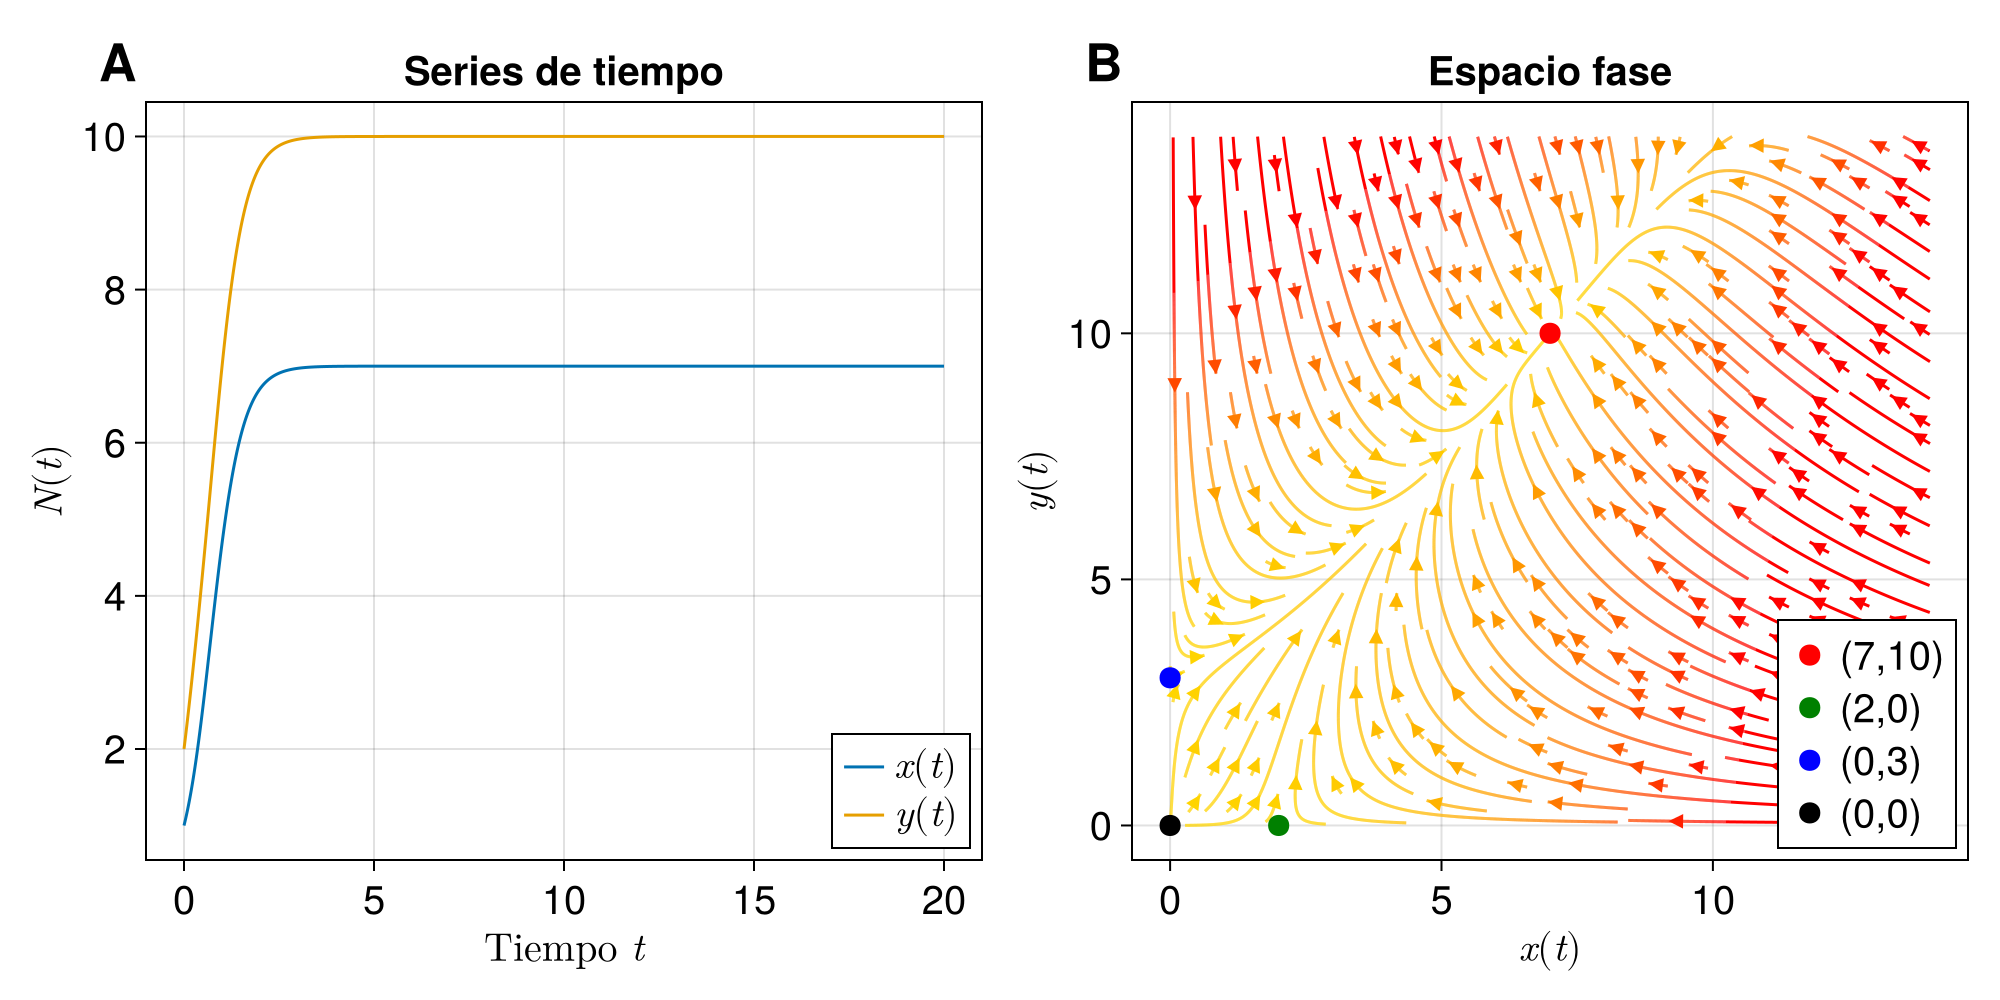
\includegraphics[scale=0.24]{../Imagenes/Cooperacion de especies}
		\caption{Sistema de Lotka-Volterra con interacciones de cooperación dados por las ecuaciones (\ref{eqn:Sist2x2Coop}). \textbf{A}) Series de tiempo del sistema para las especies $x(t)$ y $y(t)$ bajo la condición inicial $(1,2)$. (\textbf{B}) Espacio fase del sistema con sus puntos fijos asociados, se muestra solamente un único punto fijo estable.}
		\label{fig:CooperacionEspecies}
	\end{figure}
	 Esto es cuanto menos interesante porque la cooperación entre las especies $x$ y $y$ es de tal forma que superan su propia capacidad de carga que funge como límite que les impone el sistema. Bajo este escenario el concepto de la capacidad de carga toma otro significado: ahora será un parámetro que regule el crecimiento de las especies, cuanto mayor sea la capacidad de carga más difícil serán sus crecimientos, sin embargo, si la capacidad de carga no es lo suficientemente grande como para contener las interacciones de cooperación entonces el crecimiento podría darse de forma desmedida de modo que todo el sistema sea completamente inestable.\\
	 \\
 	La cooperación entre especies fomenta su crecimiento y ahora su estabilidad se posiciona en puntos que quedan por arriba de sus capacidades de carga. Algo similar ocurre para el comensalismo (-0) y el amensalismo (+0), solo que una de las especies seguirá un comportamiento logístico lo cual indica que no sufre algún impacto mientras que la otra especie se ve beneficiada o perjudicada dependiendo de la interacción que tenga. Para la interacción de depredación $(+-)$ la especie depredadora se beneficia mientras que la presa se ve perjudicada.
 	\newpage
 	Ahora modificamos el sistema (\ref{eqn:Sist2x2Coop}) de tal modo que obtengamos cada una de estas interacciones. En este caso se elige que $\alpha_{21}=0$ de la ecuación $\dot{y}$ y $\alpha_{12}=\pm\frac{1}{2}$ de la ecuación $\dot{x}$ para cubrir los casos de comensalismo y amensalismo. La ecuación $\dot{y}$ queda reducida a una ecuación logística normal y pese a la dinámica que ocurra con $\dot{x}$, no se ve afectada y mantiene su estabilidad en su capacidad de carga. 
 	\begin{figure}[h!]
 		\centering
 		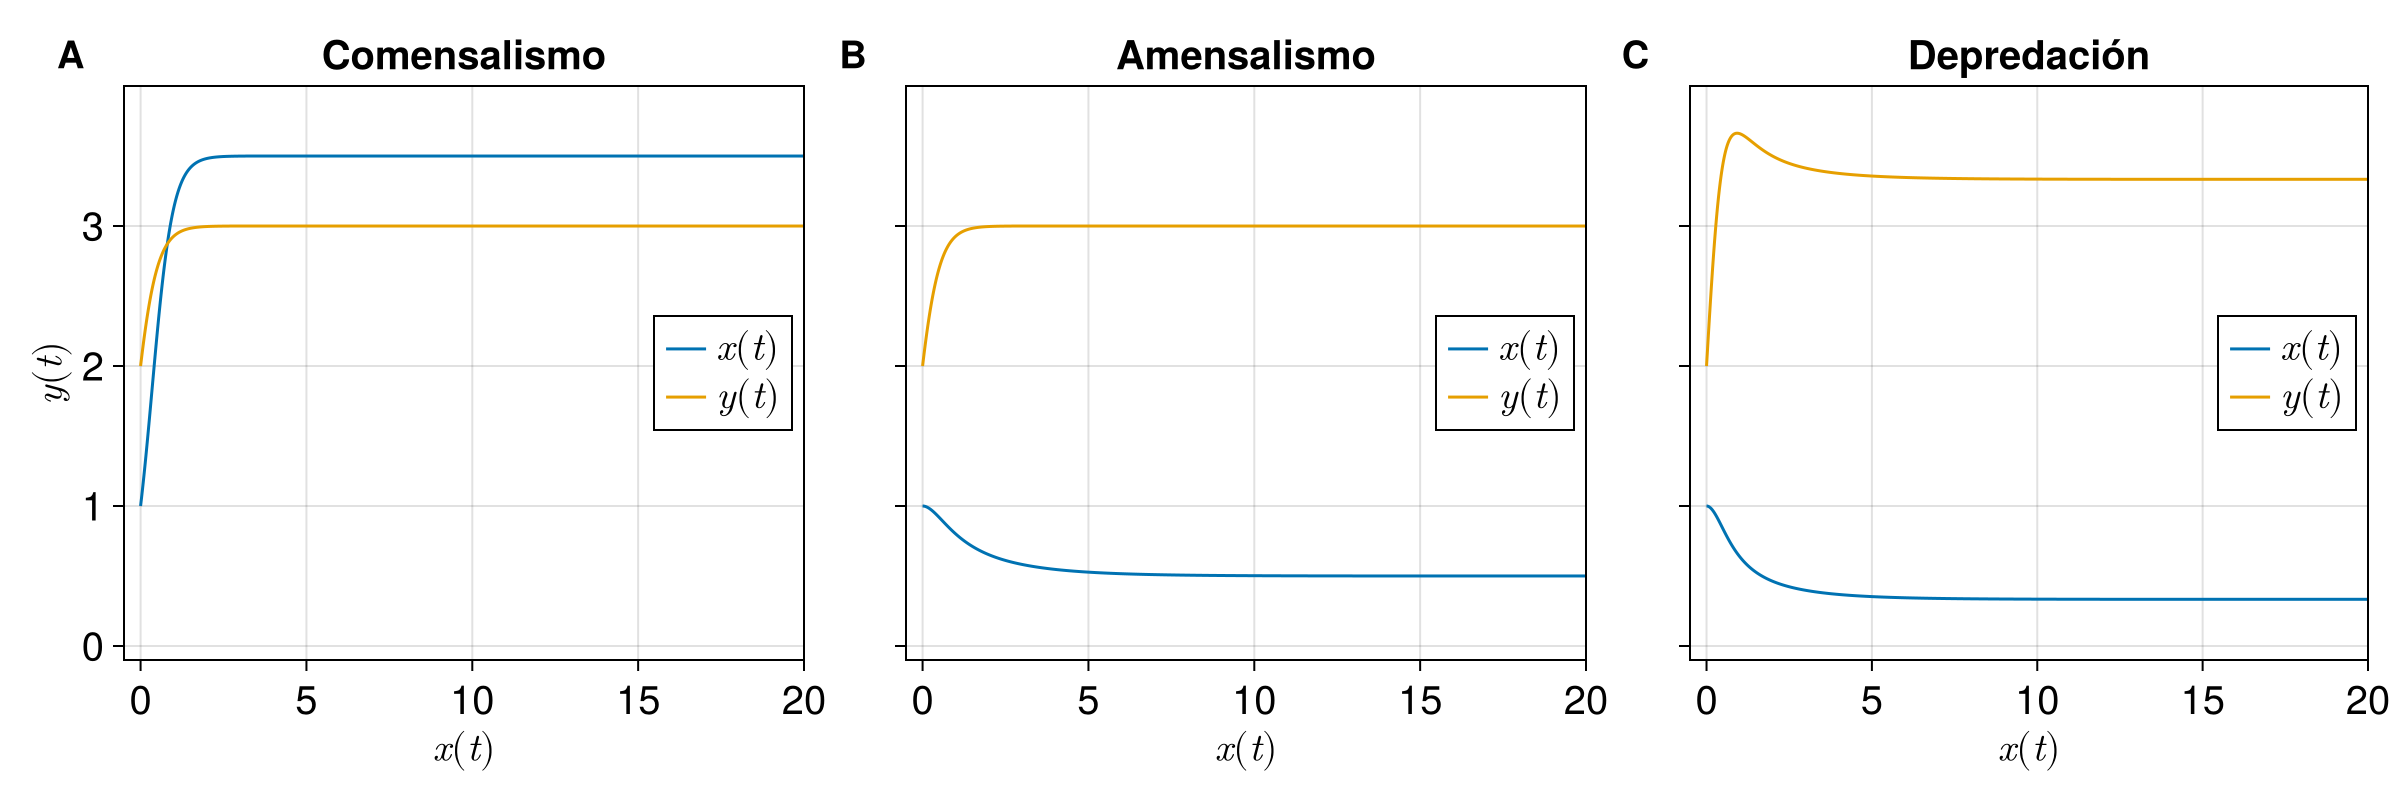
\includegraphics[scale=0.2]{../Imagenes/STrestoInteracciones}
 		\caption{Series de tiempo para las interacciones comensalismo, amensalismo y depredación. (\textbf{A}) Para el comensalismo se definió $\alpha_{21}=0$ y $\alpha_{12}=-\frac{1}{2}$. (\textbf{B}) Para el amensalismo se consideró $\alpha_{21}=0$ y $\alpha_{12}=\frac{1}{2}$ (\textbf{C}) Para la depredación se consideró $\alpha_{21}=-1$ y $\alpha_{12}=\frac{1}{2}$.}
 		\label{fig:RestoInteraccionesST}
 	\end{figure}
	La especie $x(t)$ es la que se verá impactada por sus coeficientes de interacción correspondientes, cuando recibe un beneficio podemos notar como es capaz de estabilizarse en un valor superior al de su capacidad de carga, mientras que en el caso contrario se ve perjudicada pero al menos no decae a $0$ su población, sino que se establece en un valor menor a su capacidad de carga correspondiente. El caso de depredación es como una combinación de los anteriores, mientras una de las especies se ve beneficiada, logra estabilizarse en un punto superior a la capacidad de carga mientras que para la especie que se ve perjudicada se establece igualmente en algún punto menor a su capacidad de carga pero sin llegar a extinguirse. Por último es importante remarcar que los pesos de la forma $\alpha_{ij}<0$ deben estar soportados por sus capacidades de carga, de lo contrario el sistema será inestable y sus soluciones divergerán.
\end{ejemplo}

\setlength{\parindent}{0cm} El lector hasta ahora quizás se haga las siguientes preguntas ¿Por qué son necesarios los autoenlaces y por qué deben de ser $\alpha_{ii}=1$ para toda $\alpha_{ii}\in\Lambda$? Se han fijado los pesos de los autoenlaces a $w=1.0$ ¿Podrán ser de otra forma? La respuesta es \textit{depende}; en los ejemplos \ref{eg:2x2} y \ref{eg:2x2CoopyDemás} hallamos una gran pista que nos resuelve esta conjetura: en estos sistemas se han separado los términos en donde tenemos por un lado el carácter logístico del sistema y por el otro lado las interacciones con las otras especies. \\
\\
Recordando la discusión que se tuvo sobre la ecuación logística (\ref{eqn:EqLogistica}) en el capítulo pasado, se mencionaba que para cierto tiempo $t^*$ en donde $N(t^*)=K$, la población llegaba a su tope de crecimiento y en ese valor se estabilizaba. El numerador del término $\frac{N}{K}$ bien puede tener un factor $c$ (tal que se tenga $\frac{cN}{K} $) y al final la capacidad de carga estará ahí para definir el tope, la cuestión es como debe  de ser $c$. Para no tener tantos problemas hacemos $c=1$, sin embargo si $c>0$ esto provocará que el valor de la capacidad de carga se modifique de modo que la población se estabilizará en algún otro punto diferente de $K$, pero a final de cuentas se estabilizará. Si $c=0$ entonces tenemos la ecuación (\ref{eqn:CrecimientoExponencial}) y ya sabemos que toda solución de esa ecuación diferencial diverge. Y si $c<0$ entonces la ecuación resultante tendrá un término de la forma $rx_i\left (1+\frac{x_i}{K_i}\right )$ el cual también va a diverger para $t\to\infty$. Por lo tanto, por motivos de simplicidad escogemos el peso de todas las $\alpha_{ii}$ como $w=1.0$. \\
\\
En resumen, las auto-interacciones en la red de incidencias son necesarias para regular el crecimiento de cada especie, este es el trabajo del término logístico que tiene cada $x_i$. Sin embargo ese atuo-regulamiento no es todo poderoso pues como se vio anteriormente, las interacciones $\alpha_{ij}$ son clave para determinar si el sistema es estable o no. Hasta ahora tenemos todo lo necesario para poder construir e integrar el sistema (\ref{eqn:LK}) de forma numérica, para ello basta únicamente con implementar correctamente el método RK4 (sec. \ref{sec:RK4}) y aplicarlo para poder obtener las series de tiempo, espacios fase y demás elementos que servirán para el análisis riguroso de lo que viene. En la sección (\ref{sec:poblacionesLK}) se muestra la implementación computacional de este sistema.

\section{Jacobiano del sistema: Matriz de interacciones}

Anteriormente se ha comentado sobre el método de la \textit{linealización} para poder acceder a matrices de interacciones de forma local alrededor de algún punto fijo. Se definió el \textit{Jacobiano} del sistema (ec. \ref{eqn:Jacobiano}) para efectuar esta tarea y más tarde se determinó el Jacobiano para el caso particular de un sistema de $N=2$ (ec. \ref{eqn:Jacobiano2}). En esta sección nos tocará hablar sobre la matriz de interacciones para un sistema de $N$ especies, se verán las interacciones resultantes y si se aplican con las interacciones de May [cita\footnote{cita}] y se abrirá paso a hablar sobre la estabilidad de este sistema.\\
\\
Recordando la definición \ref{def:LKVectorial} se define el sistema de Lotka-Volterra generalizado bajo la función vectorial $\mathbf{F}:\mathbb{R}^n\to\mathbb{R}^n$ donde se tienen las especies como dominio y las funciones de su dinámica en el codominio. Para determinar el Jacobiano de $\mathbf{F}(\vec{x})$ tenemos que aplicar la derivada $i$-ésima a cada $f_i(\vec{x})\in\mathbf{F}(\vec{x})$ para ello separamos en dos casos, para cuando elementos de la diagonal: $\frac{\partial f_i(\vec{x})}{\partial x_i}$, y para elementos fuera de la diagonal: $\frac{\partial f_i(\vec{x})}{\partial x_k}$; tomamos las ecuaciones del sistema (\ref{eqn:LK}) para realizar el cálculo:
$$
f_i(x) = r_ix_i\left (1-\frac{\sum_{j=1}^N \alpha_{ij}x_j}{K_i}\right )
$$
para los términos de la diagonal tenemos
\begin{equation}\label{eqn:Jacobiano_ii}
	\begin{split}
			f_i(\vec{x}) &= r_ix_i - \frac{\sum_{j=1}^N r_i\alpha_{ij}x_ix_j}{K_i} \\
			\frac{\partial f_i(\vec{x})}{\partial x_i} &= r_i -
			\frac{2\alpha_{ii}x_i+\sum_{j\neq i} r_i\alpha_{ij}x_j}{K_i}\\
			\frac{\partial f_i(\vec{x})}{\partial x_i} &= r_i \left (1-\frac{2x_i+\sum_{j\neq i}\alpha_{ij}x_j}{K_i}\right )
	\end{split}
\end{equation}
y para los términos que quedan fuera de la diagonal tenemos
\begin{equation}\label{eqn:Jacobiano_ij}
		\frac{\partial f_i(\vec{x})}{\partial x_k} = -\frac{r_i\alpha_{ik}x_i}{K_i} 
\end{equation}
\begin{definición}
	Sea $\mathcal{I}\in\mathcal{M}_N(\mathbb{R})$ donde $N$ es el número de especies del sistema de Lotka-Volterra generalizado. Definimos la matriz de \textit{interacciones} del sistema de Lotka-Volterra generalizado de la siguiente forma\footnote{La implementación computacional del Jacobiano la puedes consultar en la sección ()}:
	\begin{equation}
		\mathcal{I}=\begin{cases}
			\mathcal{I}_{ii} = r_i \left (1-\frac{2x_i+\sum_{j\neq i}\alpha_{ij}x_j}{K_i}\right ),\qquad&\text{para }i\in\{1,...,N\}\\
			\mathcal{I}_{ij} = -\frac{r_i\alpha_{ik}x_i}{K_i},\qquad&\text{para }i\neq j
		\end{cases}
	\end{equation}
\end{definición}
Una vez hallando el/los punto(s) fijo(s) del sistema y evaluándolo(s) en $\mathcal{I}$ tendremos finalmente un sistema lineal al que le podemos calcular sus eigenvalores para determinar su estabilidad. A primera vista se puede notar que los coeficientes de $\mathcal{I}$ voltean el signo con respecto de la matriz de incidencias $\Lambda$, esto parece ajustarse perfectamente con las interacciones de May en donde se discutía que tienen signos opuestos con respecto de la red de incidencias; de momento esto aplica únicamente para los elementos fuera de la diagonal. ¿Qué ocurre con los elementos de la diagonal?
\begin{proposición}
	Los elementos de la diagonal de la matriz de interacciones $\mathcal{I}$ son negativos, es decir:
	$$
	r_i \left (1-\frac{2x_i+\sum_{j\neq i}\alpha_{ij}x_j}{K_i}\right )<0
	$$	
	\begin{proof}
		Revisando los términos de la ecuación comenzamos por $r_i$, sabemos que corresponde con la tasa de crecimiento y que forzosamente debe ser mayor que cero para estimular el crecimiento de las $x_i$. Por lo que realmente debemos demostrar que lo que esta entre paréntesis es menor que cero, es decir:
		$$
		1-\frac{2x_i+\sum_{j\neq i}\alpha_{ij}x_j}{K_i}<0\qquad\Longleftrightarrow\qquad K_i<2x_i+\sum_{i\neq j}\alpha_{ij}x_j
		$$
		Esto implica que para que la derivada parcial de los elementos de la diagonal sean menores que cero, se debe de cumplir que la suma de las interacciones de la especie $x_i$ con las especies $x_j$ (incluido $2x_i$) debe ser mayor a la capacidad de carga de la especie $x_i$, o sea $K_i$. Esto ya lo habíamos visto en el Ejemplo \ref{eg:2x2CoopyDemás} (ver $\mathbb{J}_{(7,10)}$) en donde las interacciones de cooperación (en este caso las negativas) propician que estabilidad de $x_i$ quede por arriba a de la capacidad de carga, es decir que cuando la estabilidad de $x_i$ es mayor que $K_i$ (sin que tiendan a infinito) entonces los valores de la diagonal de la matriz de interacciones $\mathcal{I}$ serán negativos.
	\end{proof}
\end{proposición}
La conjunción de todo esto nos dice que los valores de autoregulación de la matriz de incidencias (que son autointeracciones positivas que limitan el crecimiento) pasan a ser interacciones de competencia $(--)$ en la martiz de interacciones. Para el resto de las entradas ocurre exactamente lo mismo, las interacciones de cooperación $(--)$ en la matriz de incidencias $\Lambda$ pasan a ser interacciones de cooperación $(++)$ en la matriz de interacciones $\mathcal{I}$, y aplicará de la misma forma para las otras cuatro interacciones posibles de modo que finalmente hemos llegado a comprobar las interacciones de May.\\
\\
¿Pueden los valores de la diagonal ser mayores que cero? La respuesta es sí, pero eso implicaría que las interacciones de $x_i$ con el resto de las especies deben ser menores a su respectiva capacidad de carga $K_i$ y esto únicamente se va a cumplir para cuando se tengan puros coeficientes positivos en la matriz de incidencias $\Lambda$, es decir, para cuando se tengan puras interacciones de competencia que no permitan que la estabilidad se posiciones por arriba de $K_i$. Más adelante se analizará este resultado y se verán sus implicaciones.\\
\\
Otra de las preguntas importantes sería ¿Cómo determinar el punto fijo \textbf{estable} de un sistema $N$-dimensional? Este autor llegó a considerar que mediante la implementación del método numérico Newton-Rhapson generalizado a un vector de dimensión $N$ sería la solución, sin embargo definir la condición inicial puede llevarte a puntos fijos que no necesariamente son estables e incluso dicha elección puede no llegar a converger oportunamente. Resulta poco práctico esta forma y sin embargo en el Ejemplo \ref{eg:2x2CoopyDemás} nuevamente hallamos una pista para la solución. Si nos fijamos en las serie de tiempo de los sistemas que propusimos integrar numéricamente (fig. \ref{fig:CooperacionEspecies} (\textbf{A}) y la fig. \ref{fig:RestoInteraccionesST}) podemos notar la convergencia hacia el punto fijo estable, de manera provechosa ¡al integrar numéricamente estamos obteniendo el punto fijo estable que necesitamos para evaluar en la matriz de interacciones $\mathcal{I}$! Lo único que restaría hacer es guardar la última iteración de nuestro conjunto solución y listo.\\
\\
No obstante, los sistemas no siempre serán estables. Dependiendo de los parámetros $p$ y $\sigma$ para la matriz de incidencias, tendremos situaciones en donde el sistema sea estable o donde no lo sea y por consiguiente (y de manera obvia) no obtengamos ningún punto fijo, por lo que esta extracción solamente será valida mientras el sistema y sus interacciones propicien que sea estable. Esto será de demasiada utilidad ya que al realizar la implementación computacional del Jacobiano, extraer el punto fijo de las series de tiempo y evaluarlo para así obtener la matriz de interacciones y averiguar su estabilidad mediantes sus eigenvalores (poniendo a prueba nuevamente la proposición \ref{prp:Atractores}). En la sección (\ref{sec:Jacobiano}) se encuentra la implementación computacional del Jacobiano considerando al punto fijo estable.